%! Licence = CC BY-NC-SA 4.0

%! Author = mariuszindel
%! Date = 30. Jan 2022
%! Project = Cheat-Sheet-Web-Engineering-3

\section{Angular}

$\bullet$Flexibles SPA-Framework für CRUD-APP
$\bullet$Dependency Injection Mechanismus
$\bullet$schnelle, JS-optimierte 2-way-binding
$\bullet$Klar strukturiert, multiple levels of abstraction
$\bullet$Erhöht Test- / Wartbarkeit client Code
$\bullet$Routing Modularität

\subsection{Angular Architecture}
$\bullet$ \textbf{ngModules} Zusammenhängender Code (Namespace in C\#)
$\bullet$ \textbf{Directives} Komponente ohne View
$\bullet$ \textbf{Component} [Controller] $\rightarrow$ Property Binding zu Template
$\bullet$ \textbf{Template} [View] HTML $\rightarrow$ Event Binding zu Component
$\bullet$ \textbf{Metadata} beschreibt Klasse
$\bullet$ \textbf{Services} [Model] Logik Komponente

\subsection{Angular Modules (ngModule)}
Basis für Angular Modularitätssystem. Module exportieren features (directives, services), andere können nutzen.
%Module können Untermodule beherbergen.
%Alle öffentlichen TS-Mitglieder werden als ein gesamtes \textit{barrel} exportiert.
ngModule ist logischer Block aus mehreren verknüpften TypeScript-Modulen (ngModule-Deklaration) in TypeScript-Modul:
\begin{lstlisting}[style=JavaScript]
@NgModule({
 declarations: [], //view classes belong to this
 imports: [ CommonModule ], //other modules needed
 exports: [ Module1 ], //declarations usable by other
 providers: [], //Services (Dependency Injection)
 bootstrap: [AppComp]}) //Main app view->Only in root
export class CoreModule { }
\end{lstlisting}

\textbf{forRoot-Import:} (in App/Root Module)
\begin{itemize}
    \item konditioniert Dienste zur gleichen Zeit
    \item Dienste genau einmal global instanziiert.
    \item Keine Konfiguration erforderlich: tree shakable providers verwenden \texttt{\tiny \{ providedIn: 'root'\}}
\end{itemize}
\textbf{forChild-Import:} (in Feature, Shared Module)
\begin{itemize}
    \item Konfiguration Diensten aktuelle Modulebene
    \item Verwenden um fremde Modul zu konfigurieren
\end{itemize}

\subsubsection{Module Types}
\textbf{Root-Modul} (oder App-Modul) $\rightarrow$ immer da!
\begin{itemize}
    \item Root-Modul wird gestartet um App zu booten.
\end{itemize}
\textbf{Core Module:} Hält Root-Modul sauber
\begin{itemize}
    \item Vom Root-Modul verwendeten components / directives / pipes
    \item Global verwendete services deklarieren
    \item Nur vom Root-Modul importiert
\end{itemize}
\textbf{Shared Modules:} Stellt global verwendete components / directives / pipes zur Verfügung
\begin{itemize}
    \item globales UI-Komponenten-Modul
    \item hier keine app-wide Singleton-provider
\end{itemize}
\textbf{Feature Modules:} Grenzen zwischen features
\begin{itemize}
    \item Domain Mod: UI speziell für Domäne
    \item Routing Mod: Legt Routing-Konfig fest
    \item Service Mod: Bietet Utility-Dienste
    \item Widget Mod: components, directives und pipes available für externe Module zur Verfügung
    \item Lazy Mod: Lose geladene Funktionsmodule
\end{itemize}

\subsection{Components}
Verwaltet View und bindet Daten aus Modell
\begin{itemize}
    \item \textbf{Controller} (App logic), TS Class mit \texttt{\tiny @Component} decorator
    \item \textbf{HTML file}, visual interface (HTML / template expression)
    \item \textbf{(S)CSS file}, styles behind HTML
\end{itemize}
$\bullet$ Tag-Name Selektoren sollten mit Anwendungsweiten Präfix beginnen wegen Kollisionen
$\bullet$ Kann verschachtelt werden $\rightarrow$ Component tree.
$\bullet$ Bereitstellung von \textbf{Information Hiding.}\
$\bullet$ Komponenten müssen innerhalb des enthaltenden Moduls deklariert werden, damit ihr \textbf{selector} für alle $\bullet$ Unterkomponenten dieses Moduls registriert wird.
$\bullet$ können exportiert werden

\subsubsection{Component Lifecycle}
\begin{minipage}{0.65\linewidth}
Wichtigste events sind
\textbf{ngOnInit} (Creation / Hydration)
\textbf{ngOnDestroy} (Destruction / Dehydration).
\textbf{ngAfter...} events hauptsächlich für Entwickler, um Sub-Components und deren DOM zu kontrollieren
Jedes interface hat eine single hook method, prefixed mit \texttt{\tiny ng}.
Interface (\textbf{OnInit} contains method \texttt{\tiny ngOnInit}).
\end{minipage}
\begin{minipage}{0.31\linewidth}
    \begin{center}
        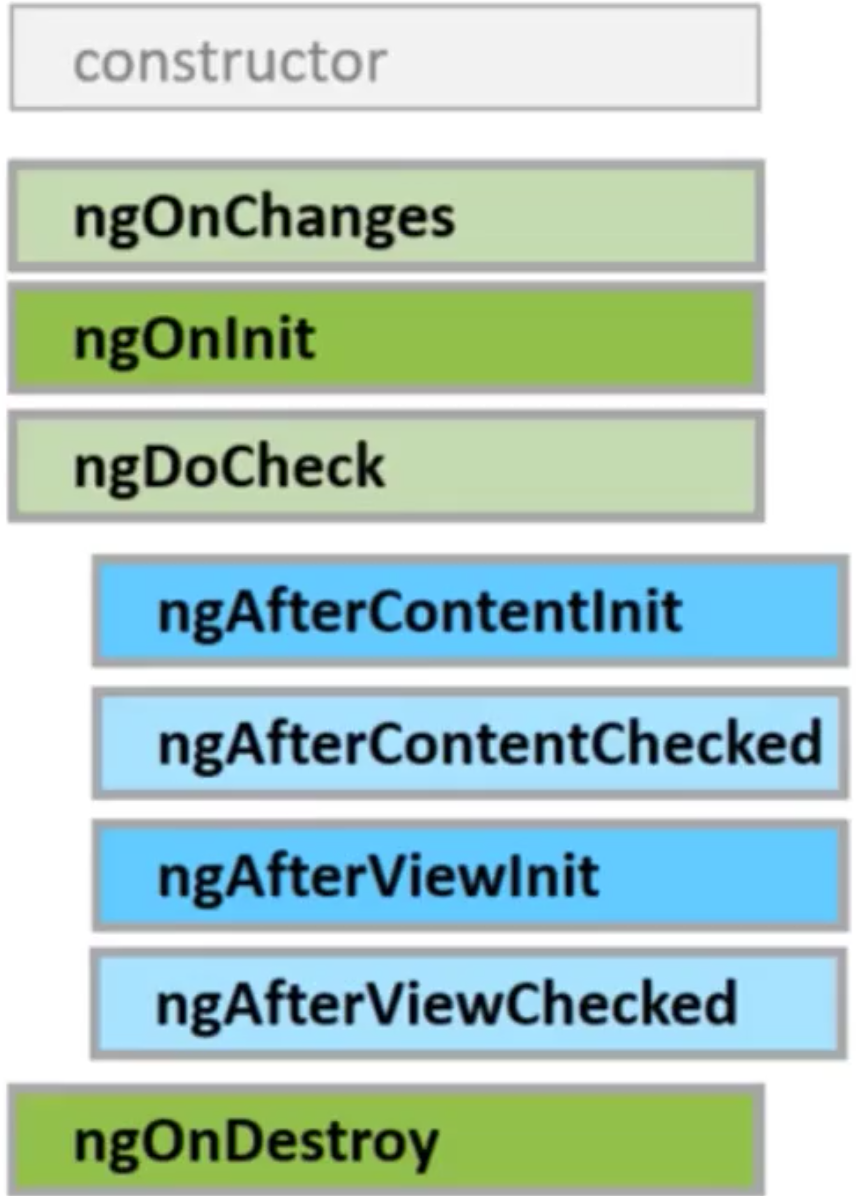
\includegraphics[width=1.1\linewidth]{./img/04-angular/component_lifecycle}
        \vspace{-8pt}
    \end{center}
\end{minipage}

%TODO: What is that exactly?!
\subsubsection{Content Projection \& Component Transclusion}
Component Transclusion und Content Projection beschreiben dieselben Konzepte
\begin{lstlisting}[style=HTML]
<ng-content select='[wed-title]'></ng-content>
<ng-content select='menu'></ng-content>
<!--£<h1 wed-title></h1> ... <menu>...</menu>£-->
\end{lstlisting}

\subsection{Templates (View in MVC)}
Angular \textbf{erweitert HTML5} mit:
$\bullet$Interpolation: \texttt{\tiny \{\{...\}\}}
$\bullet$ Template Expression/Statements
$\bullet$ Binding Syntax
$\bullet$ Directives
$\bullet$ Template Reference Variables
$\bullet$ Template Expression Operators

\subsubsection{Binding \& Interpolation}
Interpolation Properties müssen \texttt{\tiny public} sein!\\
\textbf{Two Way Binding:}
\begin{lstlisting}[style=HTML]
<input [(ngModel)]="counter.team" />
\end{lstlisting}
\textbf{Event Binding:} From View to Model
\begin{lstlisting}[style=HTML]
<button (click)="counter.eventHandler($event)">
\end{lstlisting}
\textbf{Property Binding:} From Model to View
\begin{lstlisting}[style=HTML]
<p>{{counter.team}}</p>
<img [attr.alt]="counter.team" src="team.jpg">
\end{lstlisting}
\textbf{Binding Ziele} müssen als Eingänge oder Ausgänge deklariert werden:
\begin{lstlisting}[style=JavaScript]
@Component({...})
export class NavigationComponent {
    @Output() click = new EventEmitter<any>();
    @Input() title: string; }
\end{lstlisting}
%TODO: Why you need I/O?

\subsubsection{Directives}
Ähnlich zu Component, aber ohne template. TypeScript class mit \texttt{\tiny @Directive()} function decorator
\textbf{Attribute Directives:}
Ändert das Aussehen / Verhalten von Element, component, directive. Als Attribut auf Host-Element anwenden
\begin{lstlisting}[style=HTML]
<!-- NgStyle -->
<div [style.font-size]="big ? 'big':'small'"></div>
<!-- NgClass -->
<div [class.special]="isSpecial"></div>
\end{lstlisting}
\textbf{Structural Directives:}
Ändert DOM Struktur (hinzufügen/löschen von Elementen)
Als Attribut auf Host-Element anwenden Ein Asterisk (*) steht vor dem directive attribute Namen
\begin{lstlisting}[style=HTML]
<div *ngIf="hasTitle"></div>
<li *ngFor="let elements of elements"></li>
\end{lstlisting}
\textbf{NgTemplates:}
nicht direkt gerendert (directive / component benötigt)
Über \texttt{\tiny \#id} referenzieren
\begin{lstlisting}[style=HTML]
<ng-template #toRef> hello </ng-template>
<div *ngIf="hasTitle; else toRef"> world </div>
\end{lstlisting}

\subsubsection{Template Reference Variables}
Verweist auf ein DOM-Element innerhalb eines Templates. Kann auch ein Referenz auf eine Komponente oder Directive sein.
\# deklariert eine Referenzvariable
\begin{lstlisting}[style=HTML]
<input placeholder="079 123 45 67" #phone>
<button (click)="call(phone.value)">Call</button>
\end{lstlisting}

\subsection{Services}
Bietet einen beliebigen Wert, Funktion, Feature. Typische Dienste: logging service, data service, message bus, tax calculator, usw.\\
\textbf{Strongly related to DI:} Angular verwendet DI, um Komponenten mit Services zu versorgen. Dienste innerhalb des DI-Containers registrieren.
\begin{lstlisting}[style=JavaScript]
@Injectable ({ providedIn: 'root' })
export class CounterService { /* ... */ }
\end{lstlisting}
\texttt{\tiny providedIn: 'root'}: Service für ganze Anwendung

\subsection{Angular Forms}
Ist externes ngModule (namens FormsModule)
Kombination aus mehreren Diensten und Direktiven (\underline{ngModel}, \underline{ngForm}, \underline{ngSubmit})\\
\textbf{Template-driven forms:}
Angular Template-Syntax mit formularspezifischen Direktiven und Techniken. Weniger Code, aber Validierungslogik in HTML (nur kleine Formulare)
\begin{lstlisting}[style=HTML]
<form> <input type="text" class="form-control" pattern="[a-zA-Z]{3,}"></form>
\end{lstlisting}
\textbf{Reactive / model driven forms:}
Import ReactiveFormsModule. Formular innerhalb des Controllers (FormBuilder). Validierung ebenfalls Teil des Controllers (leichter zu testen)
\begin{lstlisting}[style=HTML]
<input type="text" class="form-control" id="name"
    required [(ngModel)]="model.name" name="name"
    #nameField="ngModel">
<div [hidden]="nameField.valid || nameField.pristine"
 class="alert alert-danger"> Name is required </div>
\end{lstlisting}

\subsection{Data Access}
Implementiert asynchronisms durch RxJS-Bibliothek. RxJS ist eine third-party welche Observable-Pattern implementiert. Ein Observable kann in ein Promise umgewandelt werden.\\
\textbf{Hot Observables:} Sequenzen von Ereignissen (Mausbewegungen / Börsenticker). Gemeinsame Nutzung durch alle Subscriber. Postfix hot-observables mit einem \texttt{\tiny \$}\\
\textbf{Cold Observables:} Werden bei Subscribe gestartet (z.B. asynchrone Webanfragen). Werden nicht unter den Subscriber geteilt. Werden automatisch geschlossen, wenn der Task beendet
\begin{lstlisting}
var subscription = this.http.get('api').subscribe(
function (x) {/* onNext -> data received (in x)*/},
function (e) {/* onError -> the error (e) thrown*/},
function () {/* onCompleted->stream closing down*/});
\end{lstlisting}

\subsection{Routing}
Externes, optionales NgModul namens RouterModule. Kombination Services und Directives: RouterOutlet, RouterLink, RouterLinkActive\\
\textbf{Defining Routes:} Der Router muss mit einer Liste von Route definitionen konfiguriert werden, Jede bildet eine Route auf eine Komponente ab.
\textbf{.forRoot():} einmal auf Root-Ebene Routen deklarieren
\begin{itemize}
    \item enthält alle directives, angegebenen Routen und den Router service selbst
    \item Jede App eine Singleton-Instanz des Routers
\end{itemize}
\textbf{.forChild():} Bei Deklaration von Subroutings
\begin{itemize}
    \item enthält alle Direktiven \& angegebenen Routen
\end{itemize}
\begin{lstlisting}[style=JavaScript]
@NgModule({
  imports:[ RouterModule.forRoot(appRoutes) ],
  exports: [ RouterModule ] })
export class AppRoutingModule {}
\end{lstlisting}
Jedes ngModule definiert eigenen Routen:
\begin{lstlisting}[style=JavaScript]
@NgModule({
  imports: [ RouterModule.forChild(welcomeRoutes) ],
  exports: [ RouterModule ] })
export class WelcomeRoutingModule {}
\end{lstlisting}
\textbf{Router Outlet:} Directive von the Router module. Legt fest, wo Router Ansichten anzeigt
\begin{lstlisting}
<router-outlet></router-outlet>
\end{lstlisting}
\textbf{Route Configuration:}\\
Router arbeitet nach Prinzip ,,first-match-wins``
\begin{lstlisting}
const appRoutes: Routes = [
 {path: 'hero/:id', component: 'Hero'},
 {path: '', redirectTo: '/home', pathMatch: 'full'},
 {path: '**', component: PageNotFound} ];
\end{lstlisting}
\textbf{Lazy Loading Configuration}\\
Module nach Bedarf (lazy load) Laden
\begin{lstlisting}[style=JavaScript]
{ path: 'config',
  loadChildren: () => import('./cfg/cfg.module')
  .then(m => m.CfgModule),
  canLoad: [ AuthGuard ] }
\end{lstlisting}

\subsection{Architecture Evaluation}

\subsubsection{MVC+S}
\textbf{Observable Business Data Service:}
Stellt Daten für mehrere Teile der App in stream-ähnlichen Weise bereit. Observable bereitgestellt. Caches business objects.\\
\textbf{RxJS Subject:}
Kernstück eines observable service.
\underline{EventEmitter<T>}
leitet sich von Subject ab. Hot Observable / liefert nicht neuesten Wert\\
\textbf{Behaviour Subject:}
Gibt Ausgangszustand aus. Speichert Daten / gibt bei Änderung \textit{next()}-Ereignisse. Nicht für Service-API offengelegt.\\
\textbf{Data Resources:}
Rückgabe kalter Observables. Muss in Hot Observable umwandeln: (\texttt{\tiny share()})

\subsubsection{Flux Architecture}
Von Facebook. Erzwingt unidirektionalen Datenfluss. Eher ein pattern als formales framework.

\subsubsection{Redux Architecture}
\textbf{ngrx:} implements the Redux pattern using RxJS.
\textbf{Vorteile:}
\begin{itemize}
    \item Verbessert Debugging, Testbar-, Wartbarkeit
    \item Undo/Redo einfacher implementiert werden
    \item Reduzierter Code in Angular-Komponenten
\end{itemize}
\textbf{Verpflichtungen:}
\begin{itemize}
    \item Zusätzliche 3rd party Biblio erforderlich
    \item Komplexere Architektur
    \item Geringere Kohäsion, globaler Zustand kann UI-/business data enthalten
    \item Datenlogik in mehreren effects/reducers
\end{itemize}

\subsection{UI Advanced}

\subsubsection{Pipes}
\begin{lstlisting}
<p>{{counter.team | uppercase}}</p>
<p>{{counter.team | uppercase | lowercase}}</p>
<p>{{counter.date | date:'longDate'}}</p>
\end{lstlisting}
\textbf{Pure-Pipes:} ausgeführt, wenn pure change der input expression feststellt. Implementiert als pure Funktionen. Eingeschränkt, aber schnell.\\
\textbf{Impure-Pipes:} Bei jedem component change detection cycle einer ausgeführt (jeder Tastendruck). Caching um Verarbeitungszeit verkürzen\\
\textbf{Predefined-Pipes:} (Datum, Zahl, Währung, async)
Angular bietet aufgrund der schlechten Performance keine Filter- / OrderBy-Pipes an.\\
\textbf{Custom-Pipes:} Mit \texttt{\tiny @Pipe()} dekorierte Klasse. Implementiert Methode \textit{transform()} des Interface \texttt{\tiny PipeTransform}. Muss zu den Deklarationen des aktuellen Moduls hinzugefügt werden.\\
\textbf{Async Pipes:} Bindet Observables direkt an UI. Änderungen automatisch verfolgt. subscribes und unsubscribes automatisch von observable.

\subsubsection{View Encapsulation}
\textbf{Component Styles:}
Apps werden mit Standard-CSS gestylt. Das CLI transponiert SCSS in CSS. Selektoren der Styles einer Komponente gelten nur innerhalb dieser Vorlage.\\
\textbf{Special Selectors:}
$\bullet$ \textit{:host} - Target styles in Element, das die Komponente hostet
$\bullet$ \textit{:host-context} - Sucht nach einer CSS-Klasse in einem Vorgänger des Host-Elements\\
\textbf{Controlling View Encapsulation:}
$\bullet$ \textit{Native:} Verwendet nativer shadow DOM des Browsers
$\bullet$ \textit{Emulated:} Emuliert das Verhalten von shadow DOM, indem es das CSS vorverarbeitet (und umbenennt)
$\bullet$ \textit{None:} keine view encapsulation (scope rules) angewendet. Alles CSS zu globalen Style hinzugefügt.

